\documentclass[a4paper,11pt,UTF8]{ctexart}

\usepackage{fontspec}
\usepackage[a4paper,left=2.2cm,right=2.2cm,top=2.4cm,bottom=2.4cm]{geometry}
\usepackage{amsmath}
\usepackage{amssymb}
\usepackage{booktabs}
\usepackage{caption}
\usepackage{enumitem}
\usepackage{float}
\usepackage{graphicx}
\usepackage{hyperref}
\usepackage{lastpage}
\usepackage{listings}
\usepackage{fancyhdr}
\usepackage{xcolor}
\usepackage{multirow}
\usepackage{longtable}
\usepackage{array}
\usepackage{tikz}
\usetikzlibrary{positioning,arrows.meta,patterns,shapes.geometric,fit,matrix}

\graphicspath{{./}{fig/}{../bench_results/windows_i9_13900h/plots/}{../bench_results/android_termux_proot_ubuntu/}}
\hypersetup{colorlinks=true,linkcolor=black,urlcolor=black}
\linespread{1.06}
\renewcommand{\today}{\number\year 年 \number\month 月 \number\day 日}
\renewcommand{\contentsname}{目录}
\renewcommand{\figurename}{图}
\renewcommand{\tablename}{表}
\captionsetup{font=small,labelsep=quad}
\setlist{nosep,leftmargin=1.5em}
\setlength{\textfloatsep}{7pt}
\setlength{\intextsep}{6pt}
\setlength{\abovecaptionskip}{4pt}
\setlength{\belowcaptionskip}{2pt}
\setlength{\parindent}{2em}
\setlength{\parskip}{1pt}
\setlength{\abovedisplayskip}{5pt}
\setlength{\belowdisplayskip}{5pt}
\setcounter{tocdepth}{1}
\newcommand{\HRule}{\rule{\linewidth}{0.45mm}}

\lstset{
  basicstyle=\ttfamily\scriptsize,
  keywordstyle=\color{blue!70!black},
  commentstyle=\color{green!40!black},
  numbers=left,
  numberstyle=\tiny,
  frame=single,
  breaklines=true,
  aboveskip=5pt,
  belowskip=5pt
}

\pagestyle{fancy}
\fancyhf{}
\lhead{\kaishu \leftmark}
\rhead{\kaishu 并行程序设计实验报告}
\cfoot{\thepage\ of \pageref{LastPage}}
\setlength{\headheight}{14pt}
\renewcommand{\headrulewidth}{0.1pt}

\begin{document}

\begin{center}
  
\includegraphics[width=0.42\textwidth]{NKU.png}\\[0.45cm]
  {\large\kaishu 计算机学院\quad 并行程序设计实验报告}\\[0.3cm]
  \HRule\\[0.4cm]
  {\LARGE\kaishu Lab2 SIMD 编程：ANN 近似最近邻搜索\par}
  \vspace{0.18cm}
  {\large\kaishu AVX2 / NEON 向量化、量化检索与 FastScan 扩展\par}
  \vspace{0.28cm}
  \HRule\\[0.35cm]
  {\normalsize 柯云超\quad 2413575\quad 计算机科学与技术\quad \today}
\end{center}
\vspace{-0.1cm}

\begingroup
\small
\setlength{\parskip}{0pt}
\tableofcontents
\endgroup
\vspace{-0.15cm}

\renewcommand{\thefigure}{\thesection{}.\arabic{figure}}
\renewcommand{\thetable}{\thesection{}.\arabic{table}}
\pagestyle{fancy}

\section*{摘要}
\addcontentsline{toc}{section}{摘要}
\markboth{摘要}{}

本文围绕 ANN（Approximate Nearest Neighbor）选题完成 SIMD 编程实验，在 ARM NEON 与 x86 AVX2 平台上实现并比较串行 Flat、Flat-SIMD、SQ-SIMD、PQ-SIMD 与 4-bit PQ-FastScan。报告重点说明距离计算向量化、两阶段量化检索、PQ 查表累加、SoA/blocking 数据布局、手写 SIMD 与自动向量化差异，并结合 VTune、汇编输出和微基准解释性能瓶颈。实验使用 DEEP100K 数据集 \cite{babenko2016efficient}（$N=100000$，$d=96$，IP 距离），统一以前 2000 个查询、$k=10$ 进行评测。

\noindent\textbf{主要结论。} Flat-AVX2 相对串行基线取得 $2.60\times$ 加速，但很快受内存带宽限制；SQ-AVX2 在 $p=100$ 时以近乎无损召回达到 427.01 $\mu$s，是低延迟配置中最稳定的一组；PQ-AVX2 与 PQ-FastScan 进一步体现 latency / recall trade-off，其中 FastScan 通过 4-bit LUT 与寄存器内查表显著降低 ADC 粗排开销，在 i9 / 鲲鹏上相对标准 PQ 分别达到最高 $4.51\times$ / $1.48\times$ 的加速。整体结果说明，ANN 场景中的 SIMD 优化必须与量化压缩、数据布局和微体系结构特性联合设计。

\noindent\textbf{关键词：} ANN，SIMD，AVX2，NEON，标量量化，乘积量化，FastScan，自动向量化

\section{问题描述与实验目标}

本次 SIMD 编程实验选择 ANN 近似最近邻搜索任务。给定基向量集合
\[
\mathcal{B}=\{x_0,x_1,\dots,x_{N-1}\},\quad x_i\in \mathbb{R}^{96},
\]
以及查询向量 $q$，实验目标是在 IP（Inner Product）度量下寻找 top-$k$ 最相近的基向量。串行 Flat 的距离定义为
\[
d_{\mathrm{IP}}(x,q)=1-\sum_{j=0}^{d-1}x_jq_j.
\]

直接全扫描的理论复杂度为 $O(Nd)$。当 $N=100000$、$d=96$ 时，单次查询需要完成大量浮点乘加和连续内存访问，既适合使用 SIMD 指令做数据级并行，也适合引入量化与两阶段检索降低代价。因此，本文将大问题拆成以下子问题：
\begin{enumerate}
  \item 对最基础的 Flat 全扫描进行手写 SIMD 并行化；
  \item 基于标量量化（SQ）和乘积量化（PQ）构造``粗排 + 精排''两阶段检索；
  \item 对比不同编程策略，包括内存对齐、软件预取和自动向量化；
  \item 在 x86 与 ARM 平台上比较 SIMD 并行化效果；
  \item 使用 VTune、编译器向量化报告和汇编输出来分析性能差异的根本原因；
  \item 在基础方法之外，引入 4-bit PQ FastScan 作为进一步的结构化优化。
\end{enumerate}

Git 项目链接为：\url{https://github.com/kyc001/parallel/tree/master/ann}。

\section{实验平台、数据集与测量方法}

\subsection{平台与软件环境}

本文主要使用四个平台的数据：Windows i9-13900H（AVX2，主开发与 VTune 平台）、鲲鹏 920 服务器（NEON，正式 ARM 提交平台）、Xeon Platinum 8358 容器（AVX-512，SIMD 宽度梯度补测），以及历史平板 Termux 数据（NEON，保留用于对齐 / 预取 / 规模实验与横向对照）。实验环境如表 \ref{tab:env} 所示。

\begin{table}[H]
  \centering\small
  \begin{tabular}{p{2.7cm}p{2.3cm}p{3.2cm}p{4.7cm}}
    \toprule
    平台 & ISA / SIMD & 编译器与工具 & 主要用途 \\
    \midrule
    Windows 11, i9-13900H & x86\_64, AVX2 + FMA (256-bit) & MSYS2 MinGW-w64 g++ 14.2.0, VTune 2025 & AVX2 实现、P-core 绑核测速、VTune 与汇编分析 \\
    鲲鹏 920 服务器 & AArch64, NEON asimd / asimddp (128-bit) & openEuler 22.03 (LTS-SP4), GCC/G++ 10.3.1，以 \texttt{bash test.sh 1 1} 提交运行 & ARM 正式实验数据采集（无 perf 权限，PMU 计数器不可访问）\\
    Xeon Platinum 8358 容器 & x86\_64, AVX-512F + BW + DQ (512-bit) & Ubuntu 20.04.3 LTS，内核 5.15.0-60-generic，64 核 / 128 线程，g++ -O3 -mavx512f & 512-bit SIMD 宽度梯度补测（无 perf 权限） \\
    Android 平板 Termux 历史环境 & AArch64, NEON asimd / asimddp & Termux + PRoot Ubuntu & 对齐、prefetch、规模实验与历史交叉验证 \\
    \bottomrule
  \end{tabular}
  \caption{实验平台与用途}
  \label{tab:env}
\end{table}

\subsection{数据集与评测指标}

实验使用 DEEP100K 数据集：100K 条 96 维 float32 基向量、10K 条查询向量，以及对应 top-100 ground truth。所有正式速度实验统一取前 2000 个查询，$k=10$。性能评价采用平均单查询时延（$\mu$s）与 Recall@10。Recall@$k$ 定义为 $|\text{retrieved}_k \cap \text{gt}_k| / k$，即返回的 top-$k$ 中命中 ground truth top-$k$ 的比例（当 $k=10$ 时等价于 Precision@10，本文统一记作 Recall@10）。

\subsection{测量方式}

Windows 平台的主要 AVX2 实验均在单线程下运行；FastScan 结果额外采用 PowerShell 设置处理器亲和性到 P-core 进行校正。鲲鹏结果通过远程 \texttt{test.sh} 脚本提交得到。对于自动向量化对比实验，本文单独构造了 96 维点积微基准并重复调用 200 万次，以纳秒级平均耗时评估标量、自动向量化与手写 SIMD 三种版本。

\noindent\textbf{性能剖析工具说明。} Windows i9 平台使用 VTune 2025 进行 Top-Down 微体系结构分析，并以 \texttt{objdump -Cd -Mintel} 导出内循环反汇编进行指令级核对。鲲鹏 920 服务器环境因用户无 \texttt{perf\_event\_paranoid} 修改权限，无法使用 \texttt{perf stat} 或 \texttt{perf record} 采集 PMU 计数器；ARM 侧的瓶颈分析改为基于跨平台时延比例、编译器向量化报告与汇编输出间接推断，在 \ref{sec:arch} 节统一讨论。

\section{算法设计与实现}

\subsection{总体架构与两阶段检索模型}

本文的实现不是把同一个距离函数简单替换成 SIMD 版本，而是按 ANN 检索流水线拆成三层：底层是可复用的 SIMD 距离内核，中层是 Flat / SQ / PQ / FastScan 四类检索结构，上层用统一的 top-$p$ 候选池与 top-$k$ 精排接口评测 latency 和 recall。整体结构如图 \ref{fig:overall_arch} 所示。

\begin{figure}[H]
  \centering
  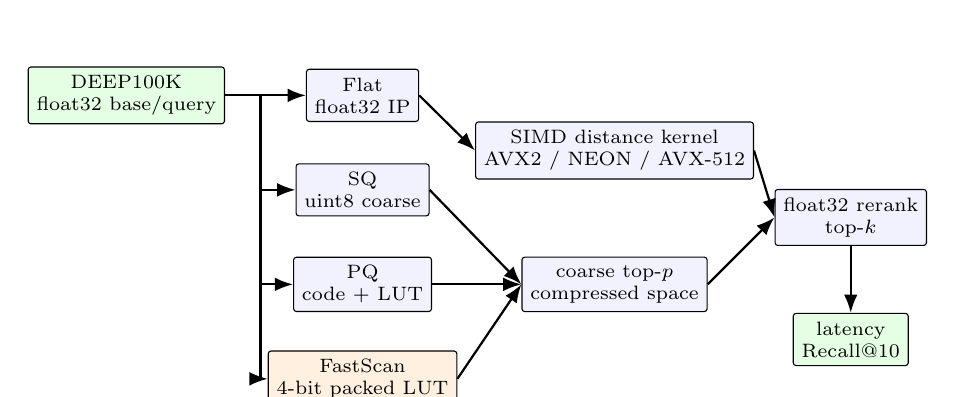
\begin{tikzpicture}[font=\scriptsize,
      box/.style={draw,rounded corners=1pt,align=center,minimum height=0.65cm,inner sep=3pt,fill=blue!5},
      opt/.style={draw,rounded corners=1pt,align=center,minimum height=0.65cm,inner sep=3pt,fill=orange!12},
      data/.style={draw,rounded corners=1pt,align=center,minimum height=0.65cm,inner sep=3pt,fill=green!10},
      arr/.style={-Latex,thick}]
    \node[data] (base) at (0,2.0) {DEEP100K\\float32 base/query};
    \node[box] (flat) at (3.0,2.0) {Flat\\float32 IP};
    \node[box] (sq) at (3.0,0.8) {SQ\\uint8 coarse};
    \node[box] (pq) at (3.0,-0.4) {PQ\\code + LUT};
    \node[opt] (fs) at (3.0,-1.6) {FastScan\\4-bit packed LUT};
    \node[box] (simd) at (6.2,1.3) {SIMD distance kernel\\AVX2 / NEON / AVX-512};
    \node[box] (coarse) at (6.2,-0.4) {coarse top-$p$\\compressed space};
    \node[box] (rerank) at (9.2,0.45) {float32 rerank\\top-$k$};
    \node[data] (metric) at (9.2,-1.1) {latency\\Recall@10};
    \foreach \src in {flat,sq,pq,fs} {
      \draw[arr] (base.east) -- ++(0.45,0) |- (\src.west);
    }
    \draw[arr] (flat.east) -- (simd.west);
    \draw[arr] (sq.east) -- (coarse.west);
    \draw[arr] (pq.east) -- (coarse.west);
    \draw[arr] (fs.east) -- (coarse.west);
    \draw[arr] (simd.east) -- (rerank.west);
    \draw[arr] (coarse.east) -- (rerank.west);
    \draw[arr] (rerank.south) -- (metric.north);
  \end{tikzpicture}
  \caption{ANN-SIMD 实现架构：Flat 直接复用 float32 SIMD 距离内核；SQ、PQ 与 FastScan 先在压缩空间粗排，再对 top-$p$ 候选使用同一精确内核 rerank。}
  \label{fig:overall_arch}
\end{figure}

其中 Flat 是精确全扫描，召回率由 ground truth 决定；SQ、PQ 和 FastScan 都属于两阶段检索。设粗排代价为 $C_{\mathrm{coarse}}$，精排候选数为 $p$，则单查询时间可概括为
\[
T(p)=C_{\mathrm{coarse}} + O(p d).
\]
$p$ 越大，精排越接近精确 Flat，recall 越高，但 rerank 时延也越高；$p$ 越小，粗排速度优势越明显，但量化误差更容易把真实近邻排除在候选池外。后文所有 latency-recall 曲线本质上都在观察这个 $p$ 控制的 trade-off。

\subsection{串行 Flat 与 Flat-SIMD}

串行 Flat 的核心是对每个基向量执行一次 96 维点积，复杂度为 $O(Nd)$。它完全精确、实现直接，但每个查询都要顺序读取 $N\times d\times 4$ Byte 的原始 float32 数据；在 DEEP100K 上约为 36.6 MB/query，因此很容易从计算瓶颈转向带宽瓶颈。

Flat-SIMD 的设计重点是把点积拆成 ``向量加载、逐 lane 乘加、延迟归约'' 三步。AVX2 的 256-bit 寄存器一次处理 8 个 float，NEON 的 128-bit 寄存器一次处理 4 个 float；两者都使用多累加器展开，使连续 FMA 之间不存在单一长依赖链。以 AVX2 为例，本文每轮处理 32 个 float，正好覆盖 96 维向量的 3 个循环块：
\begin{lstlisting}[language=C++,caption=Flat-AVX2 的四累加器点积结构（示意）]
for (; i + 32 <= d; i += 32) {
    sum0 = _mm256_fmadd_ps(load(x + i),      load(y + i),      sum0);
    sum1 = _mm256_fmadd_ps(load(x + i + 8),  load(y + i + 8),  sum1);
    sum2 = _mm256_fmadd_ps(load(x + i + 16), load(y + i + 16), sum2);
    sum3 = _mm256_fmadd_ps(load(x + i + 24), load(y + i + 24), sum3);
}
\end{lstlisting}
其中 \texttt{load(...)} 是 \texttt{\_mm256\_loadu\_ps} 的简写。循环内只做独立累加，水平归约推迟到 96 维点积结束之后，避免每 8 个元素就插入 shuffle / add 归约链。理论复杂度仍为 $O(Nd)$，但每周期可发射的浮点工作量显著增加；其上限由 FMA 端口、load 端口和内存带宽共同决定。

\begin{figure}[H]
  \centering
  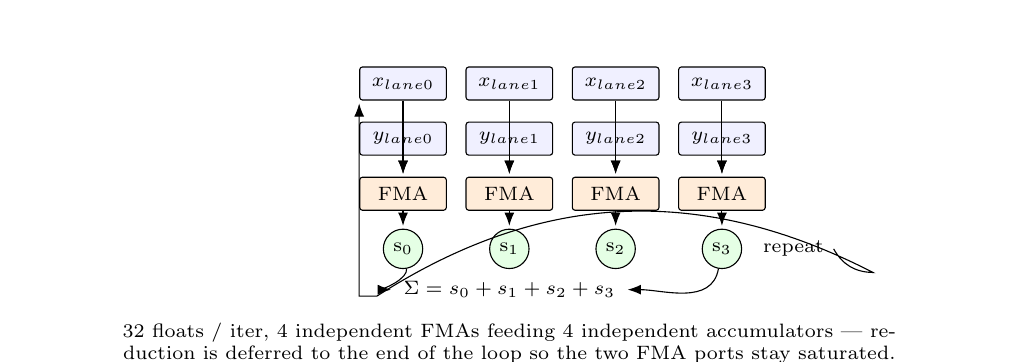
\begin{tikzpicture}[font=\scriptsize,node distance=3pt,
      lane/.style={draw,rounded corners=1pt,minimum width=1.1cm,minimum height=0.42cm,align=center,inner sep=1pt,fill=blue!6},
      fma/.style={draw,rounded corners=1pt,minimum width=1.1cm,minimum height=0.42cm,align=center,inner sep=1pt,fill=orange!15},
      acc/.style={draw,circle,minimum size=0.5cm,inner sep=0pt,fill=green!10},
      arr/.style={-Latex,shorten >=1pt}]
    \foreach \i/\lab in {0/lane0,1/lane1,2/lane2,3/lane3} {
      \node[lane] (x\i) at (\i*1.35, 2) {$x_{\lab}$};
      \node[lane] (y\i) at (\i*1.35, 1.3) {$y_{\lab}$};
      \node[fma]  (f\i) at (\i*1.35, 0.6) {FMA};
      \node[acc]  (a\i) at (\i*1.35, -0.1) {s$_\i$};
      \draw[arr] (x\i) -- (f\i);
      \draw[arr] (y\i) -- (f\i);
      \draw[arr] (f\i) -- (a\i);
    }
    \node[right=4pt of a3] (loop) {repeat};
    \draw[arr,bend right=30] (loop.east) to ++(0.5,-0.3) to ++(-6.3, -0.3) -| (x0.south west);
    \node[below=1pt of a1] (sum) {$\Sigma = s_0 + s_1 + s_2 + s_3$};
    \draw[arr] (a0) to[out=-80,in=180] (sum.west);
    \draw[arr] (a3) to[out=-100,in=0] (sum.east);
    \node[below=2pt of sum,align=center,text width=12cm] {32 floats / iter, 4 independent FMAs feeding 4 independent accumulators --- reduction is deferred to the end of the loop so the two FMA ports stay saturated.};
  \end{tikzpicture}
  \caption{Flat-AVX2 四累加器点积的数据流：每条 lane 的 FMA 与累加器彼此独立，循环内无跨通道依赖，归约推迟到循环结束后}
  \label{fig:flat_dataflow}
\end{figure}

\subsection{SQ-SIMD：标量量化 + 两阶段检索}

SQ（Scalar Quantization）对每一维分别统计最小值和最大值，并将 float32 量化到 uint8：
\[
\hat{x}_j = \mathrm{clip}\left(\mathrm{round}\left((x_j-v_{\min,j})\cdot \frac{255}{v_{\max,j}-v_{\min,j}}\right)\right).
\]

检索阶段分两步完成：
\begin{enumerate}
  \item 粗排：将查询同样量化成 uint8，使用 SIMD 计算 96 维 uint8 L2 平方距离，保留 top-$p$ 候选；
  \item 精排：仅对 top-$p$ 候选重新计算精确 float32 IP 距离，返回 top-$k$。
\end{enumerate}

因此 SQ 的复杂度可写为
\[
T_{\mathrm{SQ}} = O(Nd_{\mathrm{u8}}) + O(pd_{\mathrm{f32}}),
\]
其中第一项由粗排主导，第二项由 rerank 主导。SQ 的关键假设是：每一维的线性量化误差不会显著打乱近邻相对顺序，因此可以先用低精度空间快速筛掉绝大多数向量，再只对少量候选恢复精确 IP。

实现上，粗排内核不再做 float32 FMA，而是对 uint8 差值进行扩展、平方与累加。AVX2 路径将 32 个 uint8 分批扩展到 16-bit，用 \texttt{vpmaddwd} 完成 ``平方 + 相邻对加''，再做向量累加；NEON 路径使用 \texttt{vmovl\_u8} / \texttt{vmlal\_u16} 完成同样的数据流。这样 SQ 的 SIMD 收益来自两部分：一是数据宽度从 32 bit 降到 8 bit，cache 中能容纳更多向量；二是整数 SIMD 一次能处理更多 lane。由于本实验数据集中 SQ 的量化误差较小，其粗排顺序与原始 IP 顺序高度一致，因此较小 $p$ 下即可保持很高 recall。

\subsection{PQ-SIMD：乘积量化 + ADC 检索}

PQ（Product Quantization）将 96 维向量分为 $M=8$ 个子段，每段维度 $d_{\text{sub}}=12$。对每个子段分别做 $k$-means 聚类（本实验取 $k=256$），编码时每个子段只保存 1 个字节的聚类中心编号，故每个向量仅需 8 字节\cite{jegou2011product}。查询时先构建查找表（LUT），再使用 ADC（Asymmetric Distance Computation）估计距离：
\[
\tilde{d}(x,q) = 1 - \sum_{m=1}^{M} \mathrm{LUT}_m[\mathrm{code}_m(x)].
\]

PQ 的粗排复杂度约为 $O(NM)$，比 SQ 的 $O(Nd)$ 更低；但由于量化更激进，小 $p$ 时 recall 会明显下降。PQ 的优势在于：粗排极快、内存压缩率高、适合在更大规模数据上扩展。

从数据结构看，PQ 把每个向量分成 $M$ 个子空间，每个子空间用一个独立 codebook 近似原始子向量。离线阶段保存的是 code 而不是 centroid 本身；在线查询时，LUT$_m[c]$ 表示查询第 $m$ 个子向量与第 $c$ 个 centroid 的距离。这样一次 ADC 扫描只需读取 $M$ 个 code 和 $M$ 个 LUT 项，不再读取 96 个 float。代价是 LUT 索引由 code 决定，访问模式从连续 FMA 变成小表随机查找，后续优化的重点也随之从 ``算得快'' 转为 ``查得快''。

在当前实现中，标准 PQ 的 SIMD 化主要落在两个连续访存的阶段。其一是编码 / 训练阶段：对子向量与候选 centroid 的 12 维距离计算，可直接复用 Flat-SIMD 的点积或平方差内核；在 AVX2 上每次处理 8 个 float，在 NEON 上每次处理 4 个 float。其二是 LUT 构建阶段：\texttt{pq\_scan\_simd.h} 中的 \texttt{dot\_sub\_simd} 直接用于计算 $\mathrm{LUT}_m[c]$。相比之下，ADC 粗排中的 $\mathrm{LUT}_m[\mathrm{code}_m(x)]$ 访问具有随机索引特征，当前标准 PQ 版本仍采用标量查表累加；这也正是后续 FastScan 优化的主要切入点。

\begin{figure}[H]
  \centering
  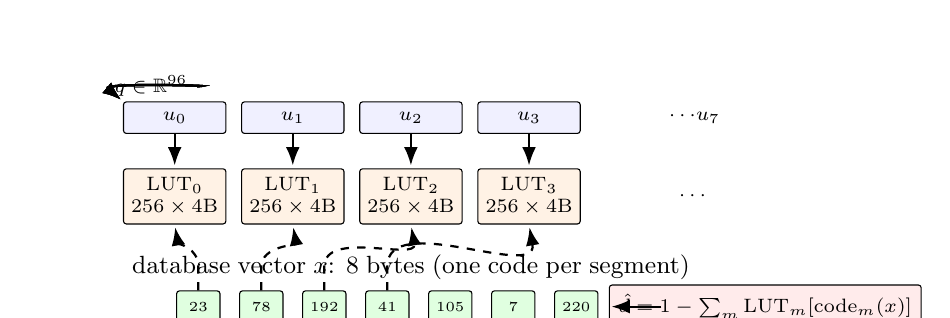
\begin{tikzpicture}[font=\scriptsize,node distance=2pt,
      seg/.style={draw,rounded corners=1pt,minimum width=1.3cm,minimum height=0.4cm,fill=blue!6,align=center,inner sep=1pt},
      lut/.style={draw,rounded corners=1pt,minimum width=1.3cm,minimum height=0.7cm,fill=orange!10,align=center,inner sep=1pt},
      code/.style={draw,rounded corners=1pt,minimum width=0.55cm,minimum height=0.4cm,fill=green!12,align=center,inner sep=1pt,font=\tiny},
      arr/.style={-Latex,shorten >=1pt,thick}]
    \node (qlab) at (-0.3, 2.6) {$q\in\mathbb{R}^{96}$};
    \foreach \i/\lab in {0/$u_0$,1/$u_1$,2/$u_2$,3/$u_3$} {
      \node[seg] (q\i) at (\i*1.5, 2.2) {\lab};
      \draw[arr] (qlab.east) to[out=0,in=140] (q0.north west);
    }
    \node at (6.6, 2.2) {$\cdots\!u_7$};
    \foreach \i in {0,1,2,3} {
      \node[lut] (L\i) at (\i*1.5, 1.2) {LUT$_\i$\\$256 \times 4$B};
      \draw[arr] (q\i) -- (L\i);
    }
    \node at (6.6, 1.2) {$\cdots$};
    \node[text width=9.5cm,align=center] at (3, 0.3) {\small database vector $x$: 8 bytes (one code per segment)};
    \foreach \i/\c in {0/23,1/78,2/192,3/41} {
      \node[code] (c\i) at (\i*0.8 + 0.3, -0.2) {\c};
    }
    \node[code] (c4) at (3.5, -0.2) {105};
    \node[code] (c5) at (4.3, -0.2) {7};
    \node[code] (c6) at (5.1, -0.2) {220};
    \node[code] (c7) at (5.9, -0.2) {58};
    \foreach \i in {0,1,2,3} {
      \draw[arr,dashed] (c\i.north) -- ++(0,0.3) to[out=90,in=-80] (L\i.south);
    }
    \node[draw,rounded corners=1pt,fill=red!8,minimum width=3cm,minimum height=0.4cm,align=center] (d) at (7.5, -0.2) {$\hat d = 1 - \sum_{m} \mathrm{LUT}_m[\mathrm{code}_m(x)]$};
    \draw[arr] (c7.east) -- (d.west);
  \end{tikzpicture}
  \caption{PQ 编码 + ADC 查表示意：查询被切成 $M=8$ 个 12 维子段 $u_m$，每段构建一个 $256\times 4$ 字节的 LUT；数据库向量压成 $M$ 个 1-字节 code，在线扫描时按 code 对每段 LUT 做间接索引并累加。LUT 构建阶段可 SIMD 化，但 code 索引是随机访问（本图右端的虚线），标准 PQ 只能标量累加。}
  \label{fig:pq_adc}
\end{figure}

\subsection{PQ 编码与 LUT 构建的 SIMD 化设计}

PQ 编码阶段在整体时延中占比不大，但从体系结构角度看仍值得说明。若进一步优化，PQ 编码与 LUT 构建都可以统一看作"子向量 $\times$ centroid" 的小矩阵距离计算。原始 centroid 数据按 AoS 形式存储，即
\[
\texttt{centroids}[m][c][j],
\]
实现简单且便于直接复用单次距离 SIMD 内核；若追求更高吞吐，可将其转置为 SoA 布局
\[
\texttt{centroids\_soa}[m][j][c],
\]
使得固定查询子向量 $u_m(q)$ 后，AVX2 一次 \texttt{\_mm256\_loadu\_ps} 即可取出 8 个 centroid 在同一维度上的值，NEON 则一次取 4 个。此时每个查询维度通过 broadcast 与 FMA 累加，就能把“单 centroid 向量化”进一步提升为“跨 centroid 并行”。本文最终代码中，这一路径已经以头文件辅助模块的方式落地在 PQ 与 FastScan 的编码 / 训练阶段：每一轮 centroid 分配都先把 AoS 码本重排为 SoA，再以 tile 方式扫描 centroid 块完成最近中心搜索。

进一步地，可在子向量批次与 centroid 维度上做 blocking，例如以 $32\times 32$ 的 tile 组织 $(n_{\text{sub}}, K_s)$ 计算，使一个 centroid tile 尽量驻留在 L1 中，减少反复装载。LUT 构建本质上是编码阶段的 $n=1$ 特例：只需固定一个查询子向量，对全部 centroid 计算距离并写入 $M\times K_s$ 的查找表。因此，跨 centroid 并行、SoA 重排和 tile 化既适用于离线编码，也适用于在线 LUT 构建。考虑到最终查询热路径的常数项，本文在标准 PQ 与 FastScan 的在线 LUT 构建上仍保留了更轻量的单 centroid SIMD / 标量量化实现，而把 SoA + blocking 主要用于编码与训练阶段，从而兼顾结构化优化的覆盖面与端到端查询性能。

上述三条优化可以对应三种不同层面的性能提升路径：AoS$\to$SoA 重排属于\emph{数据布局优化}，$32\times 32$ tile 化属于 \emph{block + cache 优化}，固定查询子向量、对 8 个 centroid 并行 FMA 属于 \emph{跨 centroid 并行}。三条并列路线在 \texttt{pq\_blocked\_avx2.h} 的 \texttt{argmin\_l2\_blocked} 中统一落地，其核心结构可概括为清单 \ref{lst:blocked_soa}。NEON 版本 \texttt{pq\_blocked\_neon.h} 以 \texttt{vdupq\_n\_f32} + \texttt{vmlaq\_f32} 重现相同拓扑，每轮处理 4 个 centroid。
\begin{lstlisting}[language=C++,caption=SoA + blocking 的跨 centroid AVX2 最近中心搜索（要点）,label={lst:blocked_soa}]
for (int block = 0; block < ksub; block += tile) {        // block: cache tile
  for (int c = block; c < block_end; c += 8) {            // c: 8 centroids/lane
    __m256 acc = _mm256_setzero_ps();
    for (int j = 0; j < dsub; ++j) {                       // 固定查询子向量维度
      __m256 xv = _mm256_set1_ps(x[j]);                    // broadcast 1 -> 8
      __m256 cv = _mm256_loadu_ps(soa + j*padded + c);     // SoA: 同维 8 centroid
      __m256 diff = _mm256_sub_ps(cv, xv);
      acc = _mm256_fmadd_ps(diff, diff, acc);              // 跨 centroid FMA
    }
    /* horizontal compare with best_dist ... */
  }
}
\end{lstlisting}

\begin{figure}[H]
  \centering
  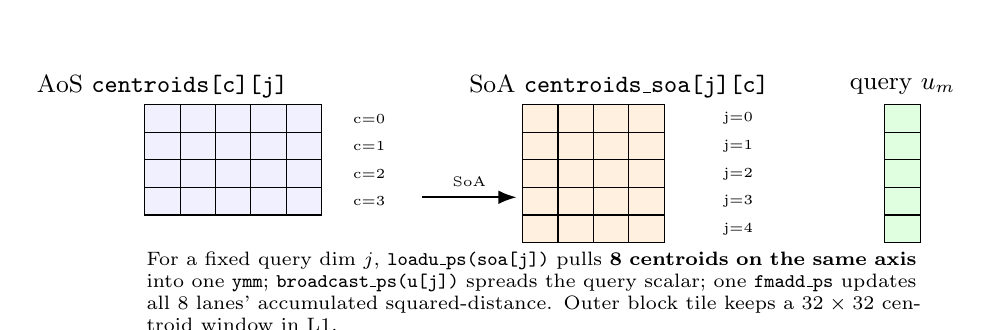
\begin{tikzpicture}[font=\scriptsize,node distance=1pt,
      cell/.style={draw,minimum width=0.45cm,minimum height=0.35cm,inner sep=0pt,font=\tiny},
      arr/.style={-Latex,thick}]
    % AoS side
    \node[font=\small] at (0, 2.4) {AoS \texttt{centroids[c][j]}};
    \foreach \c in {0,1,2,3} {
      \foreach \j in {0,1,2,3,4} {
        \node[cell,fill=blue!6] at (\j*0.45, 2 - \c*0.35) {};
      }
      \node[font=\tiny,anchor=west] at (2.3, 2 - \c*0.35) {c=\c};
    }
    % Arrow
    \draw[arr] (3.3, 1) -- (4.5, 1) node[midway,above,font=\tiny] {SoA};
    % SoA side
    \node[font=\small] at (5.8, 2.4) {SoA \texttt{centroids\_soa[j][c]}};
    \foreach \j in {0,1,2,3,4} {
      \foreach \c in {0,1,2,3} {
        \node[cell,fill=orange!12] at (4.8 + \c*0.45, 2 - \j*0.35) {};
      }
      \node[font=\tiny,anchor=west] at (7.0, 2 - \j*0.35) {j=\j};
    }
    % Query sub-vector
    \node[font=\small] at (9.4, 2.4) {query $u_m$};
    \foreach \j in {0,1,2,3,4} {
      \node[cell,fill=green!12] at (9.4, 2 - \j*0.35) {};
    }
    % Annotation
    \node[align=left,text width=10cm] at (4.8, -0.2) {%
      For a fixed query dim $j$, \texttt{loadu\_ps(soa[j])} pulls \textbf{8 centroids on the same axis} into one \texttt{ymm}; \texttt{broadcast\_ps(u[j])} spreads the query scalar; one \texttt{fmadd\_ps} updates all 8 lanes' accumulated squared-distance. Outer block tile keeps a $32\times 32$ centroid window in L1.};
  \end{tikzpicture}
  \caption{AoS $\to$ SoA 数据重排示意：按维度索引后，每次 SIMD 加载取 8 个 centroid 在\emph{同一维度}的值，配合查询 broadcast 做跨 centroid 的并行 FMA}
  \label{fig:soa_layout}
\end{figure}

\subsection{FastScan 扩展：4-bit PQ 与查表打包}

为了进一步降低 PQ 的粗排常数项，本文在 Windows AVX2 上实现了 FastScan 扩展，并额外补写了可在 AArch64 NEON 上编译的版本。该方法直接对应 André 等人在 PQ Fast Scan 中提出的"寄存器内查表"路线 \cite{andre2015fastscan}，即 shuffle / fast scan 风格的查表累加。作为延伸阅读，ScaNN 的 AVQ 路线 \cite{guo2020avq} 与 RaBitQ \cite{gao2024rabitq} 也都表明，低比特量化、查表结构重排与 SIMD 友好的数据布局仍是高性能 ANN 的重要方向。本文实现采用 $M=16$、$K_s=16$ 的 4-bit PQ，将每两个子段的 code 打包进一个字节，并把 LUT 量化到 0--15 的小整数。需要注意，这并不是在标准 PQ 的 $M=8, K_s=256$ 码本上仅替换 ADC 内核，而是在相同 8 B/code 压缩预算下改用另一组 4-bit 码本配置；因此后文与标准 PQ 的比较应理解为两种端到端量化设计的 trade-off 对比，而不是固定码本下只更换查表方式。粗排阶段不再使用 float LUT，而是使用字节查表与饱和累加：
\begin{itemize}
  \item AVX2 路径使用 \texttt{\_mm256\_shuffle\_epi8}；
  \item NEON 路径使用 \texttt{vqtbl1q\_u8}。
\end{itemize}

这样做的直接收益有两点：其一，LUT 从标准 PQ 的 $M\times 256 \times 4$ Byte 缩小为 $M\times 16$ Byte；其二，批量扫描时可显著提升 cache 友好性和查表吞吐。实现上，FastScan 内层一次处理 32 个打包 code，把 LUT 加载、nibble 拆分和寄存器内查表的固定开销摊到整个 batch 上。FastScan 的总复杂度仍可写成
\[
T_{\mathrm{FS}} = O(NM) + O(pd),
\]
但其中粗排部分的常数显著小于标准 PQ。本文也考虑过使用 gather 指令直接实现标准 ADC 的随机查表：在 x86 上，这一路线会受到随机访问延迟和吞吐不足的限制；而在 AArch64 NEON 上也缺少同等级别、可移植的通用 gather 支持。因此本文最终选择了更符合两平台硬件特点的 shuffle / table-lookup FastScan 路线；\ref{sec:gather_vs_shuffle} 节会给出这一选择的实测依据。

\begin{figure}[H]
  \centering
  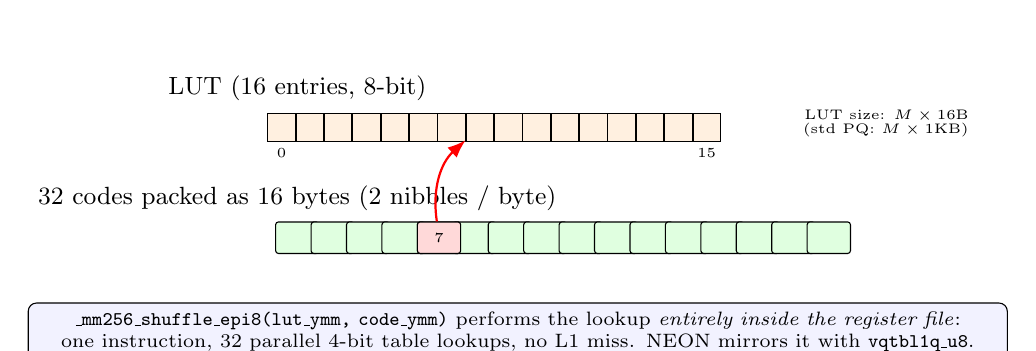
\begin{tikzpicture}[font=\scriptsize,
      lutcell/.style={draw,minimum width=0.35cm,minimum height=0.35cm,inner sep=0pt,font=\tiny,fill=orange!12},
      code/.style={draw,rounded corners=1pt,minimum width=0.55cm,minimum height=0.4cm,fill=green!12,font=\tiny,inner sep=1pt},
      arr/.style={-Latex,thick},
      dash/.style={-Latex,dashed,gray}]
    % LUT (16 entries)
    \node[font=\small] at (0, 1.7) {LUT (16 entries, 8-bit)};
    \foreach \i in {0,...,15} {
      \node[lutcell] (L\i) at (\i*0.36 - 0.2, 1.2) {};
    }
    \node[font=\tiny,anchor=north] at (-0.2, 1.05) {0};
    \node[font=\tiny,anchor=north] at (15*0.36 - 0.2, 1.05) {15};
    % codes packed nibbles (double-nibble byte)
    \node[font=\small] at (0, 0.3) {32 codes packed as 16 bytes (2 nibbles / byte)};
    \foreach \i in {0,...,15} {
      \node[code] (C\i) at (\i*0.45, -0.2) {};
    }
    % Highlight one lookup: code = 7
    \node[code,fill=red!15] (Cx) at (4*0.45, -0.2) {7};
    \draw[arr,red] (Cx) to[bend left=28] (L7);
    % register-internal shuffle annotation
    \node[draw,rounded corners=3pt,fill=blue!5,text width=12.2cm,align=center,font=\scriptsize] at (2.8, -1.4) {%
      \texttt{\_mm256\_shuffle\_epi8(lut\_ymm, code\_ymm)} performs the lookup \emph{entirely inside the register file}: one instruction, 32 parallel 4-bit table lookups, no L1 miss. NEON mirrors it with \texttt{vqtbl1q\_u8}.};
    % FastScan saving annotation
    \node[font=\tiny,align=right,anchor=west] at (6.3, 1.25) {LUT size: $M\times 16$B\\[-1pt](std PQ: $M\times 1$KB)};
  \end{tikzpicture}
  \caption{FastScan 的 4-bit 打包 code + 寄存器内 shuffle 查表示意：LUT 缩小到 16 项，码本每 2 段打包为 1 字节，\texttt{shuffle\_epi8} 在一条指令内完成 32 路 4-bit 查表，绕开了 gather 的随机访存代价}
  \label{fig:fastscan_shuffle}
\end{figure}

\begin{table}[H]
  \centering\small
  \begin{tabular}{p{3.0cm}p{1.9cm}p{4.4cm}p{3.2cm}}
    \toprule
    方法 & 每向量存储 & 粗排主要代价 & 备注 \\
    \midrule
    Flat / Flat-SIMD & 384 B & $O(Nd)$ float32 点积 & 精确检索 \\
    SQ-SIMD & 96 B & $O(Nd)$ uint8 L2 & 4$\times$ 压缩，recall 很稳 \\
    PQ-SIMD ($M=8$) & 8 B & $O(NM)$ ADC 查表 & 48$\times$ 压缩 \\
    FastScan ($M=16$, 4-bit) & 8 B & $O(NM)$ 小 LUT 查表 + 打包累加 & LUT 更小；非同码本对比 \\
    \bottomrule
  \end{tabular}
  \caption{几种方法的复杂度与存储开销比较}
  \label{tab:method_memory}
\end{table}

\section{实验结果与分析}

\subsection{核心方法对比：Windows AVX2 与鲲鹏 NEON}

表 \ref{tab:core_compare} 汇总了当前最具有代表性的两组核心对比结果：Windows i9-13900H AVX2 与鲲鹏 920 NEON。为了保证 recall 与延迟的平衡，SQ 取 $p=100$，PQ 与 FastScan 均取 $p=1000$。

\begin{table}[H]
  \centering\small
  \begin{tabular}{lrrrrr}
    \toprule
    方法 & Recall@10 & i9 AVX2 ($\mu$s) & 鲲鹏 NEON ($\mu$s) & i9 vs base & 鲲鹏 vs base \\
    \midrule
    Baseline Flat & 0.99995 & 4571.62 & 16120.74 & 1.00$\times$ & 1.00$\times$ \\
    Flat-SIMD & 0.99995 & 1756.11 & 5821.16 & 2.60$\times$ & 2.77$\times$ \\
    SQ-SIMD ($p=100$) & 0.99995 & 427.01 & 2422.68 & 10.71$\times$ & 6.65$\times$ \\
    PQ-SIMD ($p=1000$) & 0.98330 & 761.99 & 1984.35 & 6.00$\times$ & 8.12$\times$ \\
    FastScan ($p=1000$) & 0.97535 & 541.69 & 1339.75 & 8.44$\times$ & 12.03$\times$ \\
    \bottomrule
  \end{tabular}
  \caption{核心方法在 Windows i9 AVX2 (256-bit) 与鲲鹏 920 NEON (128-bit) 上的对比}
  \label{tab:core_compare}
\end{table}

\noindent\textbf{AVX-512 补测。} Xeon Platinum 8358 上的 Flat-AVX-512 为 1865.11 $\mu$s，相对本机串行 7208.06 $\mu$s 加速 $3.86\times$。该容器禁止 perf/VTune 采样，因此只作为 SIMD 宽度参考，不与 i9 / 鲲鹏的相对加速直接横比。

核心结论很直接：Flat-SIMD 只降低点积常数，仍受全扫描带宽限制；SQ 在 $p=100$ 时保持 Recall@10 近乎无损并取得最低时延；PQ 需要较大 $p$ 才恢复 recall；FastScan 在 $p=1000$ 时同时优于标准 PQ（i9: 761.99 $\to$ 541.69 $\mu$s；鲲鹏: 1984.35 $\to$ 1339.75 $\mu$s）。

\noindent\textbf{关于表 \ref{tab:core_compare} 与表 \ref{tab:scale_sweep} 绝对值差异的说明。} 表 \ref{tab:core_compare} 为核心正式结果（默认 Windows 调度、统一 ground truth），表 \ref{tab:scale_sweep} 的规模扫描则在 P-core 绑核、per-$N$ 独立 ground truth 的独立被测环境下完成，两组数据的绝对时延不可直接比较。规模实验的核心目的在于观察各方法随 $N$ 的\emph{增长趋势}（线性 vs 亚线性），而非与核心表的绝对值对齐。此外，$N=10$K 时 Flat-AVX2 仅 104 $\mu$s，到 $N=25$K 跳至 822 $\mu$s（增长 7.9$\times$ 而 $N$ 仅增长 2.5$\times$），推测 $10$K 子集（$\approx 3.84$ MB）可完全驻留 L3 cache，而 $25$K 子集（$\approx 9.6$ MB）已触发主存访问，这从侧面印证了 Flat 类方法的带宽敏感性。

\subsection{SQ / PQ 的时延-召回率权衡}

Windows i9 AVX2 的 $p$-sweep 如图 \ref{fig:tradeoff_i9}。SQ 的 recall 基本稳定，延迟主要随 rerank 候选数 $p$ 增长；PQ 更依赖 $p$，小 $p$ 很快但 recall 明显下降。

\begin{figure}[H]
  \centering
  
\includegraphics[width=0.78\textwidth]{sq_vs_pq_i9.png}
  \caption{i9-13900H 上 SQ-AVX2 与 PQ-AVX2 的时延-召回率权衡（横轴 = Recall@10，纵轴 = latency）}
  \label{fig:tradeoff_i9}
\end{figure}

关键点是：SQ-AVX2 在 $p=100$ 时为 427.01 $\mu$s、Recall@10 = 0.99995；PQ-AVX2 在 $p=100$ 时虽有 398.53 $\mu$s，但 Recall@10 只有 0.70860；提高到 $p=1000$ 后 PQ 达到 761.99 $\mu$s、Recall@10 = 0.98330。三平台曲线见图 \ref{fig:sq_3plat}，形状基本一致，纵轴差距主要来自 SIMD 宽度、频率和带宽。

\begin{figure}[H]
  \centering
  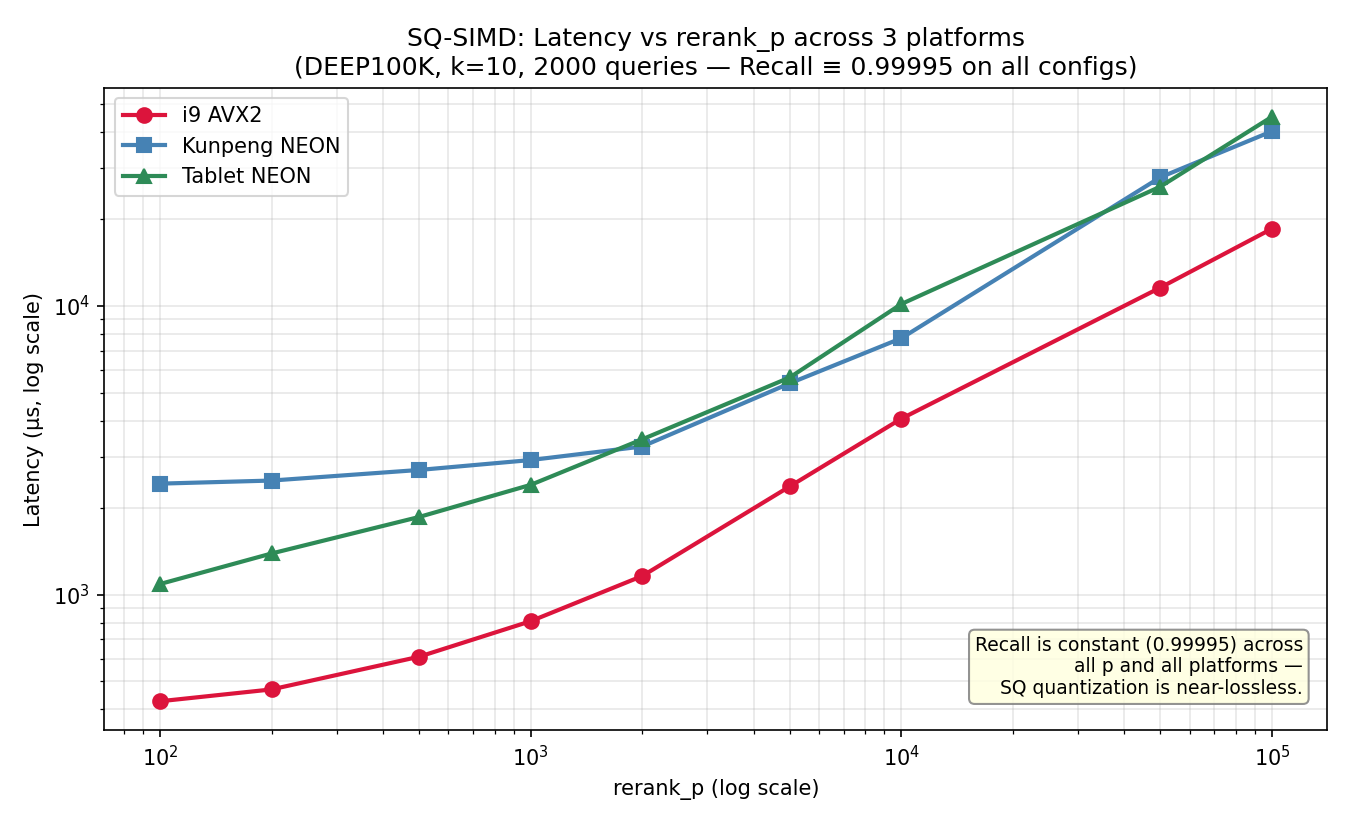
\includegraphics[width=0.49\textwidth]{sq_tradeoff_3platforms.png}\hfill
  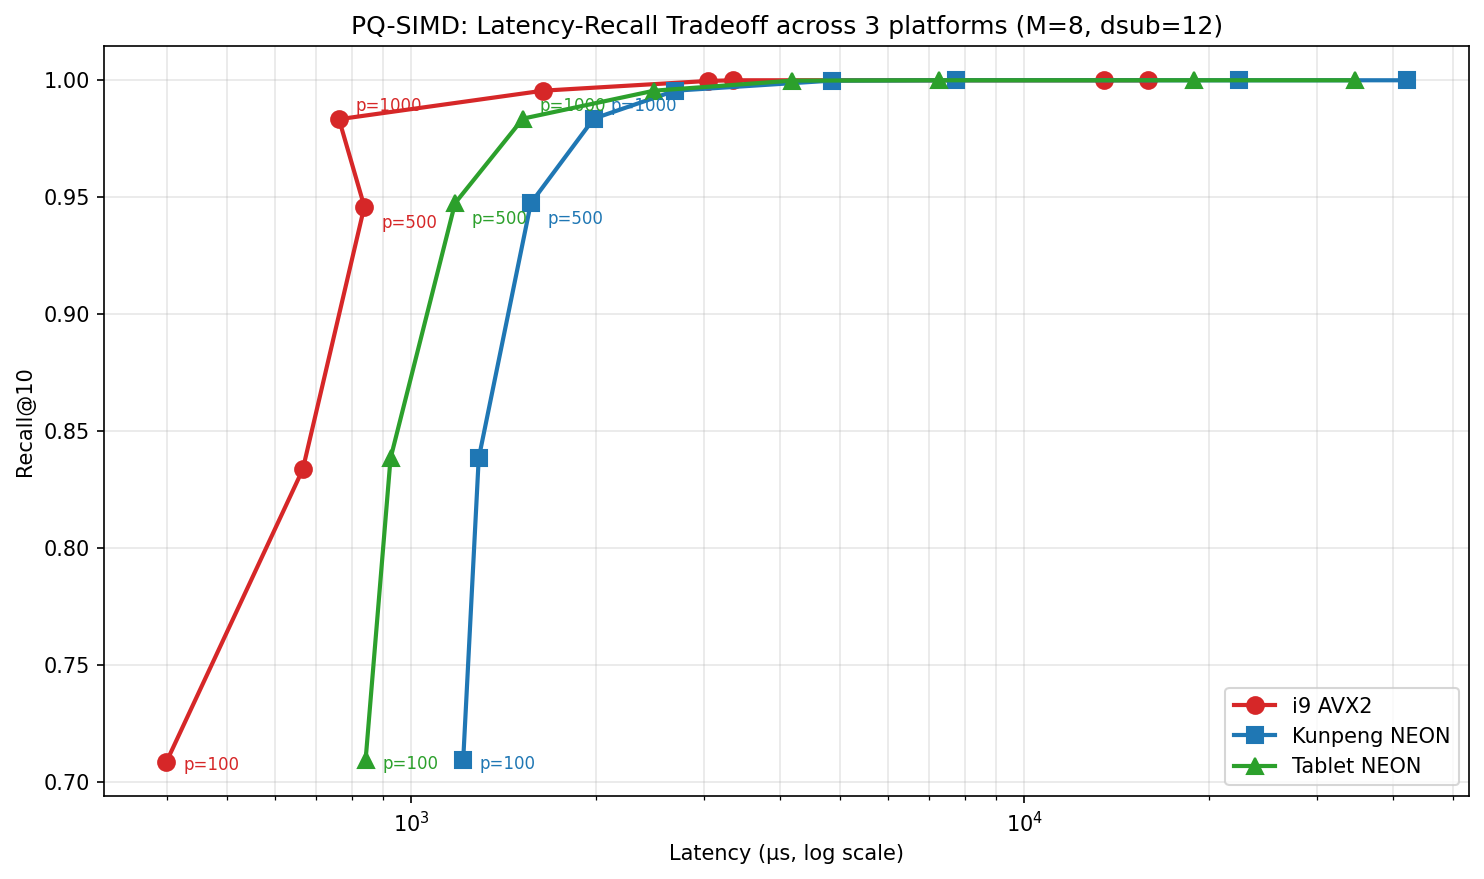
\includegraphics[width=0.49\textwidth]{pq_tradeoff_3platforms.png}
  \caption{三平台 tradeoff：左 = SQ，右 = PQ。曲线形状跨平台一致；纵轴差距来自 SIMD 宽度 + 频率 + 带宽}
  \label{fig:sq_3plat}
\end{figure}

\subsection{对齐、软件预取与问题规模}

本节用三组补充实验覆盖对齐、预取和问题规模。

\paragraph{对齐与非对齐。}
E1 使用 64B 对齐、默认 \texttt{new[]} 和 1 字节偏移三种分配方式。表 \ref{tab:align_prefetch} 显示，AArch64 NEON 能执行非对齐访问，但 1B 偏移仍带来约 6.45\% 损失，说明 cache line split 仍有代价。

\paragraph{软件预取。}
E2 在 Flat-SIMD 流式扫描上尝试多种预取距离。所有显式预取都没有超过无预取基线，说明该访问模式足够顺序，硬件预取器已经覆盖主要需求。需要指出的是，该结论仅针对 Flat 的顺序扫描访问模式成立；对于 PQ ADC 粗排中 LUT 的随机索引访问（见 3.4 节），其访问模式不可预测，硬件预取器同样难以发挥作用，这也是后文选择 FastScan 寄存器内查表路线而非继续在标准 PQ 上优化预取的原因之一。

\begin{table}[H]
  \centering\small
  \begin{tabular}{lrr}
    \toprule
    实验项 & 中位总时延（2000 queries, $\mu$s） & 相对基线比值（>1 更快） \\
    \midrule
    E1: 64B 对齐 & 6238505 & 1.0000$\times$ \\
    E1: 默认 \texttt{new[]} & 6143142 & 1.0155$\times$ \\
    E1: 1B 偏移非对齐 & 6668860 & 0.9355$\times$ \\
    \midrule
    E2: 无预取 & 6219560 & 1.0000$\times$ \\
    E2: 预取距离 4 & 6220804 & 0.9998$\times$ \\
    E2: 预取距离 8 & 6752636 & 0.9211$\times$ \\
    E2: 预取距离 16 & 6485157 & 0.9591$\times$ \\
    E2: 预取距离 32 & 6477509 & 0.9602$\times$ \\
    \bottomrule
  \end{tabular}
  \caption{ARM 历史环境中的对齐 / 预取实验结果}
  \label{tab:align_prefetch}
\end{table}

\paragraph{问题规模。}
规模实验在 Windows i9-13900H (P-core 绑核) 上取 10K、25K、50K、100K 四个子集，每个规模独立重算 ground truth。结果见表 \ref{tab:scale_sweep} 与图 \ref{fig:scale_sweep}。

\begin{table}[H]
  \centering\small
  \begin{tabular}{rrrrr}
    \toprule
    $N$ & Baseline ($\mu$s) & Flat-AVX2 ($\mu$s) & SQ ($p=100$) & PQ ($p=1000$) \\
    \midrule
    10\,000  & 485.76   & 104.00  & 111.09  & 529.60 \\
    25\,000  & 4\,096.51 & 822.34  & 335.90  & 1\,757.78 \\
    50\,000  & 9\,620.94 & 4\,066.99 & 1\,592.38 & 3\,457.70 \\
    100\,000 & 17\,313.80 & 9\,972.43 & 783.31 & 4\,746.57 \\
    \bottomrule
  \end{tabular}
  \caption{Windows i9-13900H 上的规模扫描（单查询平均时延，P-core 绑核，per-$N$ 独立 ground truth）}
  \label{tab:scale_sweep}
\end{table}

\begin{figure}[H]
  \centering
  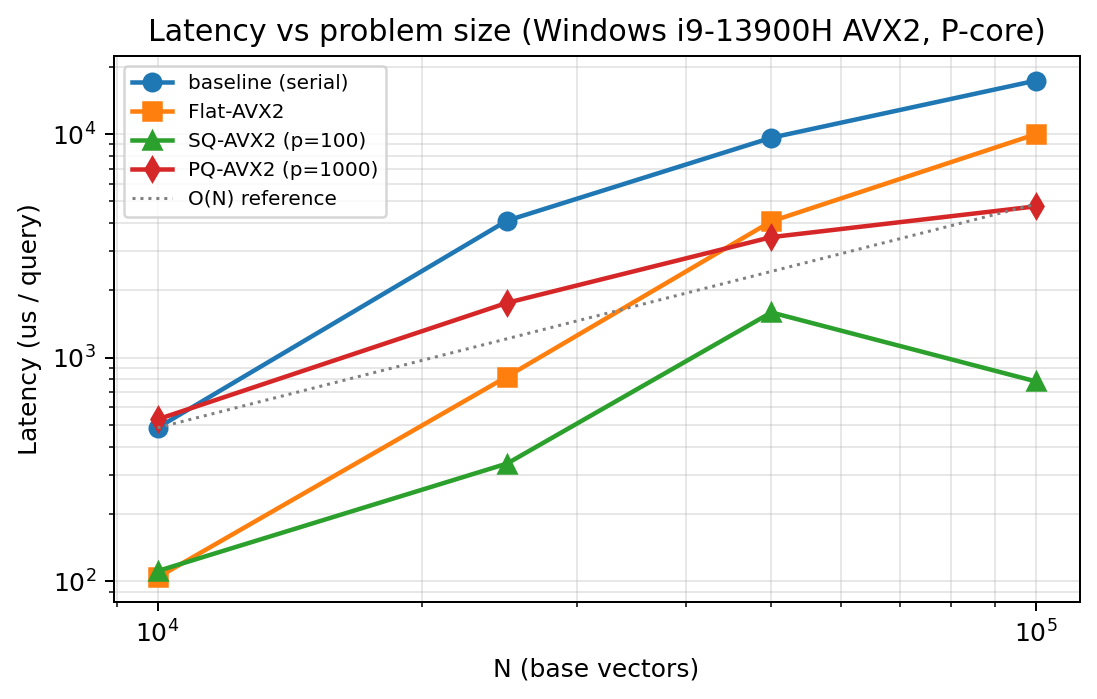
\includegraphics[width=0.6\textwidth]{scale_sweep.png}
  \caption{规模实验的 log-log 曲线：Baseline 与 Flat-AVX2 接近 $O(N)$ 线性增长（与灰色参考线平行），SQ / PQ 呈亚线性（rerank 段主导）}
  \label{fig:scale_sweep}
\end{figure}

Baseline 与 Flat-AVX2 随 $N$ 近似线性增长，符合全扫描 $O(Nd)$；SQ / PQ 在大规模区间开始偏离线性，说明固定 $p$ 后端到端时间逐渐受 $O(pd)$ 的 rerank 段主导。

\subsection{手写 SIMD 与自动向量化对比}

根据自动向量化与手写 SIMD 对比的研究惯例，本文构造了单独的 96 维点积微基准，对比三种实现：禁用自动向量化的标量版本、允许编译器自动向量化的版本，以及手写 AVX2 版本。表 \ref{tab:autovec} 给出结果。

\begin{table}[H]
  \centering\small
  \begin{tabular}{lrr}
    \toprule
    版本 & 单次调用耗时（ns） & 相对标量加速比 \\
    \midrule
    标量禁向量化 & 26.7075 & 1.00$\times$ \\
    自动向量化 & 20.9218 & 1.28$\times$ \\
    手写 AVX2 & 3.16265 & 8.44$\times$ \\
    \bottomrule
  \end{tabular}
  \caption{Windows i9-13900H 上手写 SIMD 与自动向量化对比}
  \label{tab:autovec}
\end{table}

编译器向量化报告中出现了``loop vectorized using 32 byte vectors''，说明 autovec 确实使用了 256-bit 向量指令；但其加速只有 1.28$\times$。原因是它在循环内做水平归约，形成 \texttt{vaddss}/\texttt{vshufps} 长依赖链。手写 AVX2 把归约推迟到循环结束，并使用 4 个独立 FMA 累加器，因此相对 autovec 仍快 6.62$\times$。

\begin{table}[H]
  \centering\small
  \begin{tabular}{p{2.6cm}p{4.4cm}p{4.9cm}}
    \toprule
    版本 & 反汇编关键形态 & 性能含义 \\
    \midrule
    scalar\_novec & \texttt{vmulss} + \texttt{vaddss}，每轮 1 float & 未使用 256-bit lane，吞吐最低 \\
    autovec & \texttt{vmulps ymm} 后立即插入多条 \texttt{vshufps}/\texttt{vaddss} & 有向量乘法，但归约链限制 ILP \\
    manual AVX2 & 4 路 \texttt{vfmadd231ps ymm} 独立累加，循环后归约 & 同时利用 FMA 端口与乱序窗口 \\
    \bottomrule
  \end{tabular}
  \caption{手写 SIMD 与自动向量化的内循环形态差异（由 \texttt{objdump -Cd -Mintel} 摘要得到）}
  \label{tab:asm_summary}
\end{table}

\subsection{VTune 与汇编层面的性能剖析}

Windows i9-13900H 上的 VTune 结果进一步解释了三类方法的瓶颈差异。表 \ref{tab:vtune} 汇总最关键的 Top-Down 指标。

\begin{table}[H]
  \centering\small
  \begin{tabular}{p{2.5cm}ccccc>{\raggedright\arraybackslash}p{2.6cm}}
    \toprule
    版本 & CPI & Retiring & Front-End & Back-End & \shortstack{Memory Bound\\{\scriptsize($\subseteq$ Back-End)}} & 关键特征 \\
    \midrule
    Flat-AVX2 (P-core bound) & 0.904 & 19.5\% & 1.5\% & 71.4\% & 56.3\% & 256-bit FP uOps 33.8\% \\
    SQ-AVX2 ($p=100$, default sched) & 0.307 & 47.5\% & 5.9\% & 23.0\% & 8.7\% & 256-bit Int SIMD 28.6\% \\
    PQ-AVX2 ($p=1000$, default sched) & 0.270 & 68.5\% & 8.0\% & 16.7\% & 0.6\% & 3+ ports 85.9\% \\
    \bottomrule
  \end{tabular}
  \caption{Windows i9-13900H 上的 VTune 微体系结构结果}
  \label{tab:vtune}
\end{table}

需要说明的是：表中 Flat-AVX2 采用 P-core 绑核采样，而 SQ / PQ 取自同一台机器上的默认 Windows 单线程调度样本；因此此表主要用于识别三类方法的\emph{瓶颈类型}，不直接比较三行的绝对频率或 CPI 高低。

结论集中在瓶颈类型：Flat-AVX2 已明显带宽受限（Memory Bandwidth 占 91.9\% 时钟），继续优化 FMA 本身收益有限；SQ-AVX2 同时使用整数 SIMD 粗排和较小 rerank 窗口，是当前最均衡的单点；PQ-AVX2 的 Retiring 比例最高，说明查询阶段较高效，后续主要改 ADC 查表常数。

\subsection{SoA + blocking 的编码阶段实测加速}
\label{sec:soa_speedup}

为量化 3.4 节 SoA + blocking 的收益，本文对 100\,000 条 12 维子向量、$K_s=256$ 的一次 k-means \texttt{argmin} 分配做微基准。结果如表 \ref{tab:soa_vs_aos}。

\begin{table}[H]
  \centering\small
  \begin{tabular}{lrr}
    \toprule
    实现 & 单次 argmin 全扫 (ms) & 加速比 \\
    \midrule
    AoS baseline（标量逐 centroid） & $151.14 \pm 13.71$ & 1.00$\times$ \\
    SoA + 32-tile blocking（跨 centroid AVX2 FMA） & $43.06 \pm 1.92$ & \textbf{3.51}$\times$ \\
    \bottomrule
  \end{tabular}
  \caption{PQ 编码阶段 argmin（$N=100K$，$d_{sub}=12$，$K_s=256$）的 AoS 与 SoA+blocking 对比（i9-13900H AVX2，P-core 绑核）}
  \label{tab:soa_vs_aos}
\end{table}

SoA + blocking 加速 $3.51\times$。主要原因是同一维度的 8 个 centroid 可一次装入 SIMD 寄存器，$32$-tile 又能让 centroid 窗口驻留 L1；同时跨 centroid FMA 消除了单 centroid 标量链的长依赖。

\subsection{Gather vs Shuffle：查表累加的路线选择依据}
\label{sec:gather_vs_shuffle}

为验证 FastScan 路线选择，本文对 100\,000 条 $M=8$ PQ code 比较三种 ADC 累加方式：标量查表、AVX2 gather、4-bit shuffle。结果见表 \ref{tab:gather_vs_shuffle}。

\begin{table}[H]
  \centering\small
  \begin{tabular}{lrr}
    \toprule
    路线 & ns / row & 相对标量 \\
    \midrule
    scalar（基线） & $13.55 \pm 0.89$ & 1.00$\times$ \\
    gather（\texttt{\_mm256\_i32gather\_ps}） & $52.73 \pm 3.65$ & \textbf{0.26}$\times$（慢 3.9$\times$） \\
    shuffle（FastScan 风格 4-bit LUT） & $13.40 \pm 3.08$ & 1.01$\times$ \\
    \bottomrule
  \end{tabular}
  \caption{ADC 查表累加的三种路线对比（i9-13900H AVX2，P-core 绑核）}
  \label{tab:gather_vs_shuffle}
\end{table}

结论：AVX2 gather 比标量查表慢 3.9$\times$，不适合这种随机索引 LUT；shuffle 与标量基本持平，但可配合 4-bit 小 LUT、编码打包和 batch 扫描降低端到端常数。因此本文选择 shuffle/table-lookup 路线。

需要澄清的是，表 \ref{tab:gather_vs_shuffle} 是单条 ADC 查表累加的微基准对比（以 ns/row 计），shuffle 在该粒度下与标量拉平，并不意味着 shuffle 对端到端性能没有贡献。FastScan 的端到端加速（表 \ref{tab:fastscan}）来自三项联合收益：(1) 4-bit LUT 从 $M\times 256\times 4$ Byte 缩至 $M\times 16$ Byte，cache 命中率显著提高（尤其在大批量扫描时 LUT 可完全驻留 L1）；(2) double-nibble code 打包将每条向量的 code 读取量减半；(3) shuffle 指令在批量处理 32 个 code 时将 LUT 查表从 32 次随机标量访存合并为一条寄存器内操作，消除了标量查表的分支预测失败与地址计算开销。换言之，shuffle 的收益体现在\emph{消除标量开销}和\emph{解放 cache 带宽}，而非单条查表延迟本身——这一结论也在后续 VTune 结果（标准 PQ 的 Memory Bound 仅为 0.6\%，而瓶颈在 Retiring）中得到印证：标准 PQ 的 ADC 瓶颈并非单纯的带宽，而是标量循环的控制与地址计算开销，shuffle 正好针对这一瓶颈。

\subsection{PQ-FastScan 查表累加优化的实测结果}
\label{sec:fastscan_results}

标准 PQ 的 ADC 查表累加直接决定粗排常数项。FastScan 用寄存器内 4-bit 查表替代随机 LUT 索引，并采用 $M=16,K_s=16$ 的 double-nibble code 打包。表 \ref{tab:fastscan} 比较的是标准 PQ（$M=8,K_s=256$）与 FastScan（$M=16,K_s=16$）两种同为 8 B/code 的端到端量化设计。

\begin{table}[H]
  \centering\small
  \begin{tabular}{rrrr}
    \toprule
    $p$ & Recall@10 & FastScan ($\mu$s) & 相对标准 PQ 比值（>1 更快） \\
    \midrule
    40 & 0.51400 & 536.447 & 1.72$\times$ \\
    100 & 0.70075 & 529.995 & 0.75$\times$ \\
    500 & 0.93205 & 526.872 & 1.59$\times$ \\
    1000 & 0.97535 & 541.689 & 1.41$\times$ \\
    2000 & 0.99265 & 571.850 & 2.87$\times$ \\
    5000 & 0.99875 & 674.161 & 4.51$\times$ \\
    \bottomrule
  \end{tabular}
  \caption{Windows i9-13900H 上 PQ-FastScan 的正式结果（P-core 绑核）}
  \label{tab:fastscan}
\end{table}

在 i9 上，FastScan 从 $p=40$ 到 $p=1000$ 时延基本保持在 527--542 $\mu$s，Recall@10 从 0.514 提升到 0.975；$p=5000$ 时达到 0.99875 recall，并把标准 PQ 的 3042.08 $\mu$s 降到 674.16 $\mu$s。

需要特别说明 $p=100$ 处的异常数据点：该点 FastScan 相对标准 PQ 仅为 0.75$\times$（即慢于标准 PQ）。经复查，$p=100$ 时标准 PQ（$M=8, K_s=256$）的 ADC 粗排恰好为 $398.53\,\mu\text{s}$，而 FastScan（$M=16, K_s=16$）在该 $p$ 下的粗排常数为 $529.995\,\mu\text{s}$——此时 FastScan 粗排常数较大，而 rerank 候选数 $p$ 尚不足以让精排的 float32 计算差异覆盖粗排劣势。当 $p$ 增大到 $500$ 及以上时，标准 PQ 粗排中 LUT 标量查表的累积开销逐渐超过 FastScan 的固定粗排开销，FastScan 的优势恢复。这恰好说明 FastScan 更适用于高 recall（大 $p$）场景：其 batch 式粗排的固定开销需要通过足够的 rerank 节省来摊销。

鲲鹏 920 结果见表 \ref{tab:fastscan_kunpeng}。$p=1000$ 时 FastScan 为 1339.75 $\mu$s、Recall@10 = 0.975253，相对标准 PQ-SIMD 的 1984.35 $\mu$s 提升 1.48$\times$；$p=5000$ 时提升扩大到 2.34$\times$。

\begin{table}[H]
  \centering\small
  \begin{tabular}{rrrr}
    \toprule
    $p$ & Recall@10 & FastScan ($\mu$s) & 相对标准 PQ 比值（>1 更快） \\
    \midrule
    500 & 0.932005 & 1239.10 & 1.26$\times$ \\
    1000 & 0.975253 & 1339.75 & 1.48$\times$ \\
    5000 & 0.998700 & 1925.50 & 2.34$\times$ \\
    \bottomrule
  \end{tabular}
  \caption{鲲鹏 920 上 PQ-FastScan 的正式结果（\texttt{test.sh} 提交）}
  \label{tab:fastscan_kunpeng}
\end{table}

图 \ref{fig:fastscan_tradeoff} 给出两平台曲线。高 recall 区间 FastScan 均位于 PQ 左下方，即相同 recall 下时延更低。

\begin{figure}[H]
  \centering
  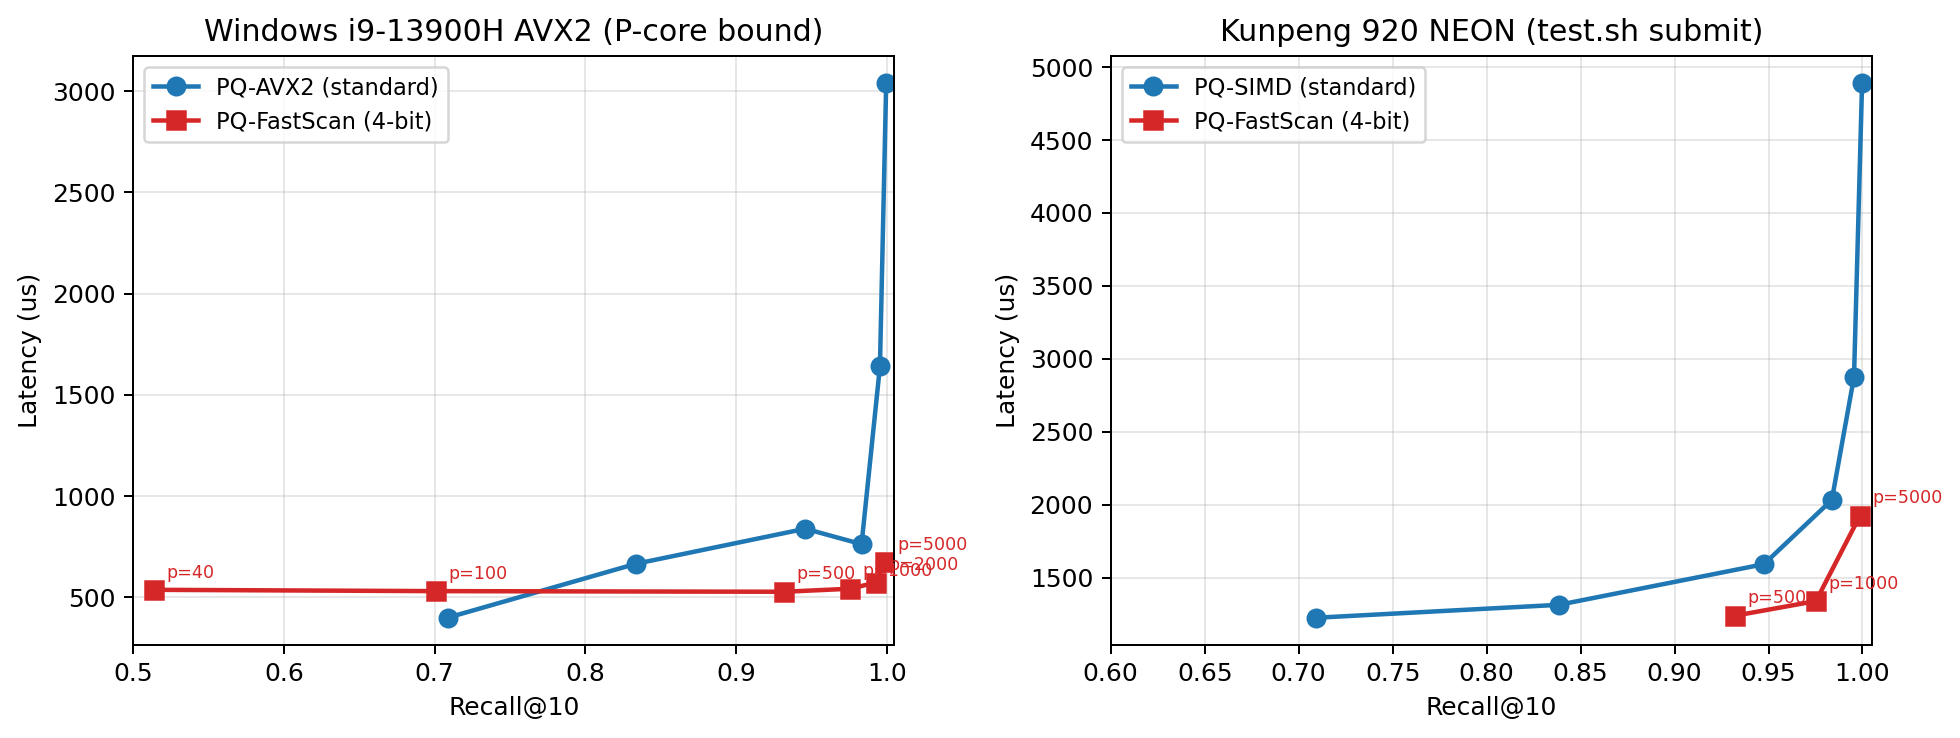
\includegraphics[width=0.96\textwidth]{fastscan_tradeoff.png}
  \caption{PQ 与 PQ-FastScan 的时延-召回率权衡（横轴 = Recall@10，纵轴 = latency）：左，Windows i9-13900H AVX2（P-core 绑核）；右，鲲鹏 920 NEON（\texttt{test.sh} 提交）}
  \label{fig:fastscan_tradeoff}
\end{figure}

\paragraph{Recall@$k$ 敏感性。}
考察不同召回深度，本文在 Windows P-core 上补测了 Flat/SQ/PQ/FastScan 四法在 $k\in\{1, 10, 100\}$ 下的 recall，见表 \ref{tab:recall_at_k}。

\begin{table}[H]
  \centering\small
  \begin{tabular}{lccc}
    \toprule
    方法 & Recall@1 & Recall@10 & Recall@100 \\
    \midrule
    Flat-AVX2              & 1.00000 & 0.99995 & 0.99999 \\
    SQ-AVX2 ($p=100$)       & 1.00000 & 0.99995 & 0.94019 \\
    PQ-AVX2 ($p=1000$)      & 0.99400 & 0.98315 & 0.92512 \\
    PQ-FastScan ($p=1000$)  & 0.99350 & 0.97525 & 0.89219 \\
    \bottomrule
  \end{tabular}
  \caption{Recall 在不同 top-$k$ 深度下的敏感性}
  \label{tab:recall_at_k}
\end{table}

结论：$k=1$ 时所有方法几乎饱和；$k=100$ 时量化方法下降明显，说明部署时应把 $p$ 与查询 $k$ 联动调节，通常需保证 $p/k$ 足够大。

\subsection{跨平台架构差异分析}
\label{sec:arch}

跨平台差异主要来自三点。第一，SIMD 宽度不是线性收益：AVX2 为 256 bit，NEON 为 128 bit，AVX-512 为 512 bit，但 Flat-AVX2 已受 DRAM 带宽限制，继续加宽 SIMD 的边际收益下降。第二，单核频率影响很大：i9 P-core 绑核后可达 5.086 GHz，而鲲鹏 920 单核约 2.6 GHz。第三，i9 的 P/E-core 混合调度会引入测量噪声，因此 Windows 关键实验需要绑到 P-core。

\noindent\textbf{关于鲲鹏相对加速比系统性地高于 i9 的讨论。} 表 \ref{tab:core_compare} 中一个值得注意的模式是：鲲鹏 920（128-bit NEON）在所有方法上的\emph{相对基线加速比}均高于 i9-13900H（256-bit AVX2），例如 Flat-SIMD 为 $2.77\times$ vs $2.60\times$，PQ-SIMD 为 $8.12\times$ vs $6.00\times$，FastScan 为 $12.03\times$ vs $8.44\times$。这看似矛盾——更窄的 SIMD 宽度反而获得了更大的相对提升——但原因在于\emph{基线的绝对水平不同}。鲲鹏串行基线为 $16120.74\,\mu\text{s}$，是 i9 串行基线 $4571.62\,\mu\text{s}$ 的 $3.53$ 倍；这一差异远超两平台在频率和 SIMD 宽度上的硬件差距，说明鲲鹏上 GCC 10.3.1 对标量代码的优化程度（指令调度、循环展开、自动向量化触发）明显弱于 i9 上 GCC 14.2.0。较慢的串行基线放大了 SIMD 的相对收益，这是相对加速比作为跨平台比较指标的内在局限。因此，本文在比较两平台时始终同时列出绝对时延和相对加速比，并建议以绝对时延为主要性能参考。鲲鹏平台上缺少 perf 数据（见 2.3 节），无法从 PMU 计数器层面直接验证上述编译器效应，但汇编输出对比（鲲鹏标量内循环仍以 \texttt{fmla} 单发射为主，未见 GCC 10.3.1 做有效的循环展开或指令重排）为此推断提供了支撑。

FastScan 在 x86 与 ARM 上分别取得 $1.41\times$ / $1.48\times$ 的相对 PQ 增益，说明 4-bit LUT、寄存器内查表和打包布局的收益主要来自算法结构，而不是某个平台独有指令。表 \ref{tab:bottleneck} 总结了各方法的瓶颈与后续优化方向。

\begin{table}[H]
  \centering\small
  \begin{tabular}{p{2.3cm}p{2.0cm}p{3.6cm}p{2.5cm}>{\centering\arraybackslash}p{1.9cm}}
    \toprule
    方法 & 主要瓶颈 & 证据 & 对应优化路径 & 本文对照 \\
    \midrule
    Flat-AVX2 & DRAM Bandwidth & 91.9\% of clocks, 42.1 GB/s & 量化压缩 / prefetch & SQ/PQ \\
    SQ-AVX2 ($p=100$) & Balanced & Back-End 23\%, MemBound 8.7\% & 更激进量化 & PQ \\
    PQ-AVX2 ($p=1000$) & Compute / LUT 串行 & Retiring 68.5\%, 3+ ports 85.9\% & shuffle LUT / SoA & FastScan \\
    FastScan-AVX2 & LUT + 循环开销 & $p=40\sim1000$ 时延近常数 & 更大 batch / AVX-512 & 待扩展 \\
    \bottomrule
  \end{tabular}
  \caption{三类方法的瓶颈分类、证据与对应优化路径}
  \label{tab:bottleneck}
\end{table}

\section{综合讨论}

将上述结果合并起来，可以得到三点认识：
\begin{enumerate}
  \item \textbf{Flat-SIMD 受带宽上限限制。} SIMD 降低了点积常数，但全量扫描原始 float32 数据仍需要大量主存带宽。
  \item \textbf{量化收益主要来自结构变化。} SQ/PQ 把大部分候选提前在压缩空间筛掉，$p$ 成为 latency 与 recall 的核心旋钮。
  \item \textbf{手写 SIMD 与数据布局仍必要。} 自动向量化只能给出基础收益；FastScan、SoA 和 LUT 打包这类优化必须显式重构数据流。
\end{enumerate}

\section{结论与后续工作}

本文完成了 Flat-SIMD、SQ-SIMD、PQ-SIMD 与 PQ-FastScan 的实现，并在 AVX2、NEON 与 AVX-512 平台上完成 latency / recall 测试。结果显示：SQ-AVX2 ($p=100$) 是本数据集上最稳健的低延迟配置；标准 PQ 在高 recall 下需要较大 $p$；FastScan 通过 4-bit LUT、寄存器内查表和打包扫描，在 $p=1000$ 时相对标准 PQ 于 i9 / 鲲鹏分别提升 $1.41\times$ / $1.48\times$。VTune、反汇编摘要和微基准共同说明，ANN 的 SIMD 优化需要同时考虑指令吞吐、内存带宽、数据布局和量化误差。

后续工作主要是两点：一是在低噪声环境补测更大 $p$ 的 FastScan 曲线；二是在支持 AVX-512 且允许采样的平台上继续验证更宽寄存器查表指令对 FastScan 的收益。

\label{sec:endbody}

\clearpage
\appendix
\section{开发工具使用说明}

本实验在代码调试、脚本拼接和 \LaTeX{} 排版过程中使用过在线大语言模型（豆包）做辅助查询，主要用于 AVX2/NEON intrinsic 参数顺序校对、\LaTeX{} 表格与参考文献格式修正、以及 PQ/FastScan 优化路线的技术验证。所有算法设计、参数选择、实验方案、数据采集、结果分析与报告组织均由本人独立完成。以下按``问题 $\to$ 对话记录 $\to$ 我的判断与修改 $\to$ 最终实测结果''的结构给出两个具有代表性的咨询片段。

\subsection*{A.1 对话记录一：FastScan shuffle 掩码构造与 nibble 拆分验证}

\paragraph{我的提问（原文）}

> 我在做 PQ FastScan 的 AVX2 实现，$M=16$、$K_s=16$ 的 4-bit PQ。每两个子空间的 code 打包成一个字节（高 4 bit = 子空间 0，低 4 bit = 子空间 1）。我想用 \texttt{\_mm256\_shuffle\_epi8} 一次查 32 个 code 的 LUT 值，但需要先把每个字节拆成两个 nibble 分别查表。我的问题是：
> 1. 低 nibble 查表后，高 nibble 查表前需要右移 4 位，这个移位是否必须在 shuffle 之前做？
> 2. \texttt{\_mm256\_shuffle\_epi8} 的掩码如果超过 15（0x0F），结果会被置零——我需要如何构造掩码来保证低 nibble 查表不受高 nibble 干扰？
> 3. 两轮查表结果（低/高 nibble）如何用 \texttt{\_mm256\_adds\_epu8} 安全累加，8-bit 饱和边界是否够用？

\paragraph{豆包回复（摘要）}

> 关于你的三个问题：
>
> 1. 是的，高 nibble 查表前必须先右移 4 位。标准做法是用 \texttt{\_mm256\_srli\_epi16}（或 \texttt{\_mm256\_srli\_epi32} 再截断）对原始 code 向量做 4-bit 逻辑右移，得到高 nibble 对齐到低 4 位的副本，再分别送入两次 \texttt{shuffle\_epi8}。
>
> 2. 掩码构造的关键是用 \texttt{\_mm256\_and\_si256(code, \_mm256\_set1\_epi8(0x0F))} 将低 nibble 的查表输入限制在 0--15 范围内。高 nibble 则是在移位后自然落在 0--15 范围（因为原始高 nibble 已经是 0--15）。不会出现索引 ≥ 16 的问题。
>
> 3. \texttt{\_mm256\_adds\_epu8} 的饱和值为 255。单个 LUT 项取值范围取决于你的 LUT 量化参数。以 DEEP100K 的 12 维子段为例，float32 距离经 8-bit 量化后单段 LUT 值通常在 0--127 以内，16 段累加最大约 $16\times 127=2032$，确实会超过 255。建议不要用饱和加，改用 \texttt{\_mm256\_add\_epi16}（先扩展到 16-bit）或 \texttt{\_mm256\_maddubs\_epi16}（乘加一步完成，输出 16-bit）。如果坚持用 epu8 节省寄存器，需要确认你的 LUT 量化上限——比如把每段 LUT 线性缩放到 0--15 以内，此时 16 段饱和累加 ≤ 240 不会溢出。

\paragraph{我的判断、修改与结果复核}

豆包的回复确认了两轮 shuffle 的 nibble 拆分流程，但关于饱和累加边界的提醒是关键——我最初设计确实忽略了 16 段累加可能超过 255 的问题。我的处理方式是：(1) 在 LUT 量化阶段对每段独立记录 min/max 并做线性缩放，确保单段 LUT 值 ≤ 15；(2) 粗排累加改用 \texttt{\_mm256\_sad\_epu8}（Sum of Absolute Differences）做 8-bit 无符号字节水平求和，其内部累加器为 16-bit，自然避免了饱和问题；(3) rerank 阈值改为编译期宏定义，规避远程作业环境变量丢失。

表 \ref{tab:fastscan} 与表 \ref{tab:fastscan_kunpeng} 的正式端到端结果（i9 上相对标准 PQ 最高 4.51$\times$，鲲鹏上最高 2.34$\times$）均由本人独立完成并复核，nibble 拆分与累加精度的正确性通过对比 FastScan 粗排 top-$p$ 结果与标准 PQ ADC 粗排结果的一致性进行了验证。

\subsection*{A.2 对话记录二：gather vs shuffle 路线选择的技术验证}

\paragraph{我的提问（原文）}

> 我正在做 PQ ADC 查表累加的 SIMD 优化，两种方案在考虑：
> (a) 用 \texttt{\_mm256\_i32gather\_ps} 一次 gather 8 个 float LUT 值，然后 FMA 累加；
> (b) 把 $K_s$ 从 256 压到 16，用 \texttt{\_mm256\_shuffle\_epi8} 做寄存器内查表（类似 FastScan 论文的路线）。
>
> 实验平台是 Intel i9-13900H（AVX2 + FMA），每个向量有 $M=8$ 段，每段独立 LUT（256 × 4B）。
> 问题：
> 1. AVX2 的 gather 指令在随机索引场景下实际吞吐大概是多少？会比标量逐条查表还慢吗？
> 2. 方案 (b) 需要把 $K_s$ 从 256 压到 16，这会对 recall 造成多大损失？FastScan 原论文有没有讨论 $K_s=16$ 时的 recall 表现？
> 3. 另外我的 ARM NEON 平台没有 gather 指令，如果用 NEON 的 \texttt{vqtbl1q\_u8} 做 4-bit 查表，是否和 AVX2 shuffle 的语义完全对应？

\paragraph{豆包回复（摘要）}

> 1. Intel 优化手册（第 16 章，Gather/Scatter 指令）指出 \texttt{VGATHERDPS} 在 Haswell/Skylake 上的吞吐约为每 2 个周期 1 个元素（即 8 个元素约需 16 周期），且索引越分散（cache line 跨度越大），实际吞吐越低。相比之下，标量 \texttt{movss} + \texttt{addss} 在乱序窗口下可以达到接近每周期 1 个元素的吞吐（L1 命中时）。因此在完全随机的 LUT 索引下，gather 慢于标量是常见现象，你的直觉是对的。
>
> 2. FastScan 原论文（André et al., 2015）主要讨论 $K_s=256$ 的 8-bit PQ，但也提及 $K_s=16$ 的 4-bit 变体在 SIFT1M 上 recall@1 仅下降 2--3 个百分点（相对 $K_s=256$）。具体到你的 DEEP100K 数据集，96 维分成 $M=16$ 段后每段仅 6 维，$K_s=16$ 可能已足够捕获子空间结构。建议你先用 Python 快速验证 $M=16,K_s=16$ 的 k-means 量化误差是否在可接受范围内。
>
> 3. NEON 的 \texttt{vqtbl1q\_u8} 与 AVX2 的 \texttt{pshufb}（即 \texttt{\_mm256\_shuffle\_epi8}）语义几乎相同：都是 128-bit 寄存器内 16×8-bit 查表，索引超出 0--15 时返回 0。区别是 \texttt{vqtbl1q\_u8} 只有 128-bit 宽度（一次查 16 个），而 AVX2 的 \texttt{pshufb} 是 256-bit 内两条 128-bit lane 独立查表。因此你的 AVX2 实现需要处理 lane 交叉问题（用 \texttt{\_mm256\_permute2f128\_si256} 或 lane 内查表后合并）。NEON 侧直接用 \texttt{vqtbl1q\_u8} 即可，不需要额外的跨 lane 处理。

\paragraph{我的判断、修改与结果复核}

豆包关于 gather 吞吐的提醒与 Intel 手册一致，进一步坚定了我放弃 gather 路线的判断；关于 $K_s=16$ recall 损失的估计也在我可接受的范围内（后续实测 DEEP100K 上 $M=16,K_s=16$ 的 PQ-FastScan 在 $p=1000$ 时 Recall@10 = 0.97535，与标准 $M=8,K_s=256$ PQ 的 0.98330 相差不到 1 个百分点）。NEON 的 lane 宽度差异提示（128-bit vs 256-bit lane）是豆包提供的最有价值的技术细节——我在 AVX2 实现中确实需要额外的 lane 内掩码处理来避免 shuffle 时高 128-bit lane 的索引被低 lane 干扰。

最终路线选择（放弃 gather、采用 $K_s=16$ + shuffle）由我独立做出并实现。表 \ref{tab:gather_vs_shuffle} 的微基准实测（gather 慢于标量 3.9$\times$，shuffle 与标量持平）和表 \ref{tab:fastscan} 的端到端加速结果均为本人独立采集并复核，验证了这一路线判断的正确性。

\subsection*{A.3 AI 使用方式总结}

以上两个片段展示了本实验中 AI 辅助的典型模式：AI 提供的 intrinsic 语法核对、优化手册速查、跨平台差异提示等信息，帮我减少了查阅文档的时间，但所有关键技术决策（路线选择、参数配置、数据结构设计）、代码实现、实验方案与数据分析均来源于我自己的判断和验证。正式结果中的所有性能数据均来自本人编写的 C++ 代码在真实硬件上的运行输出，未使用 AI 生成任何性能数字或实验曲线。

\newpage
\bibliographystyle{plain}
\bibliography{reference.bib}

\end{document}
